\documentclass[dvipdfmx,cjk,10.2pt]{beamer} 
%\documentclass[dvipdfm,cjk]{beamer} %% オプションは環境や利用するプログラムに
%\documentclass[dvips,cjk]{beamer}   %% よって変える

\usepackage{subfigure}
\usepackage[all]{xy}
\usepackage{wrapfig}

\newcommand{\C}{\mathbb{C}}
\newcommand{\D}{\mathbb{D}}
\newcommand{\R}{\mathbb{R}}
\newcommand{\Q}{\mathbb{Q}}
\newcommand{\Z}{\mathbb{Z}}
\newcommand{\N}{\mathbb{N}}

\newcommand{\Imag}{\mathrm{Im}}
\newcommand{\id}{\mathrm{id}}


\makeatletter
\newcommand\xleftrightarrow[2][]{%
  \ext@arrow 9999{\longleftrightarrowfill@}{#1}{#2}}
\newcommand\longleftrightarrowfill@{%
  \arrowfill@\leftarrow\relbar\rightarrow}
\makeatother

\AtBeginDvi{\special{pdf:tounicode 90ms-RKSJ-UCS2}} %% しおりが文字化けしないように
%\AtBeginDvi{\special{pdf:tounicode EUC-UCS2}}

\setbeamertemplate{navigation symbols}{} %% 右下のアイコンを消す
\setbeamertemplate{theorems}[normal font] %%斜体を直す

\usetheme{CambridgeUS}         %% theme の選択
%\usetheme{Boadilla}           %% Beamer のディレクトリの中の
%\usetheme{Madrid}             %% beamerthemeCambridgeUS.sty を指定
%\usetheme{Antibes}            %% 色々と試してみるといいだろう
%\usetheme{Montpellier}        %% サンプルが beamer\doc に色々とある。
%\usetheme{Berkeley}
%\usetheme{Goettingen}
%\usetheme{Singapore}
%\usetheme{Szeged}

%\usecolortheme{rose}          %% colortheme を選ぶと色使いが変わる
%\usecolortheme{albatross}

%\useoutertheme{shadow}                 %% 箱に影をつける
\usefonttheme{professionalfonts}       %% 数式の文字を通常の LaTeX と同じにする

%\setbeamercovered{transparent}         %% 消えている文字をうっすらと表示する


\theoremstyle{definition}
\setbeamertemplate{theorems}[numbered]  %% 定理に番号をつける
\newtheorem{Thm}{定理}[section]
%\theoremstyle{example}
\newtheorem{Ex}[Thm]{例}
%\newtheorem{exam}[thm]{Example}
\newtheorem{Rem}[Thm]{注意}
\newtheorem{Conj}[Thm]{予想}
\newtheorem{Def}[Thm]{定義}
\newtheorem{Prob}[Thm]{問題}

\setbeamercolor{block title}{fg=blue!70!black, bg=blue!15!white} 
\setbeamercolor{block body}{fg=black, bg=blue!10!white}



\begin{document}
\title{微分・積分 第2回} 
\author{慶応義塾大学}            %% ここに書かれた情報は色々なところに使われるので
\institute[]{総合政策学部・環境情報学部}   %% なるべく設定した方が良い
\date{}



\begin{frame}                  %% \begin{frame}..\end{frame} で 1 枚のスライド
\titlepage                     %% タイトルページ
\end{frame}

%\begin{frame}                  %% 目次 (必要なければ省略)
%\tableofcontents
%\end{frame}






%%%%%%%%%%%%%%%%%%%%%%%%%%%%%%%%%%%%%%%%%%%%%%%%%%%%%%%%%%%%%%%%%%%%%%%%%%%%%%%%%%%%%%%
%%%%%%%%%%%%%%%%%%%%%%%%%%%%%%%%%%%%%%%%%%%%%%%%%%%%%%%%%%%%%%%%%%%%%%%%%%%%%%%%%%%%%%%

\section{講義概要}


\begin{frame}
\frametitle{今日の内容}



\begin{enumerate}
\item 関数 (写像との関係, グラフ, 定義域)
\item 多項式関数, 有理関数, 無理関数, 三角関数, 指数関数, 対数関数
\item 符号関数, 床関数, 天井関数
\end{enumerate} 



記号: $\R_+=\{ x \in \R \ | \ x>0\}$, $\R_{\ge0}=\{ x \in \R \ | \ x\ge 0\}$


\end{frame}




%%%%%%%%%%%%%%%%%%%%%%%%%%%%%%%%%%%%%%%%%%%%%%%%%%%%%%%%%%%%%%%%%%%%%%%%%%%%%%%%%%%%%%%
%%%%%%%%%%%%%%%%%%%%%%%%%%%%%%%%%%%%%%%%%%%%%%%%%%%%%%%%%%%%%%%%%%%%%%%%%%%%%%%%%%%%%%%

\section{関数}

\begin{frame}
\frametitle{写像}

集合$X$の各元に対して, 集合$Y$の元を唯一つ定める対応のことを写像と呼び, $f:X \rightarrow Y$と表す. 
$X$のことを\underline{定義域}, $Y$のことを\underline{値域}という. \\
\ \\

写像$f:X\rightarrow Y$によって$x \in X$が$y\in Y$に対応するとき, $y$を$f$による$x$の\underline{像}といい, $y=f(x)$と書く. 
 %この対応を次のように書くこともある 
\vspace{-1mm}
$$
f:X \longrightarrow Y, \ \ \ x \mapsto y. 
$$

\vspace{-1mm}

 \begin{figure}[htbp]
 \begin{center} 
  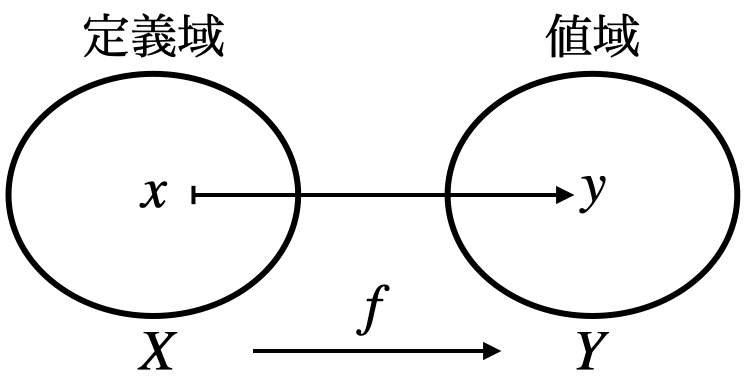
\includegraphics[width=50mm]{map.png}
 \end{center}
\end{figure}

\vspace{-1mm}

\end{frame}



%%%%%%%%%%%%%%%%%%%%%%%%%%%%%%%%%%%%%%%%%%%%%%%%%%%%%%%%%%%%%%%%%%%%%%%%%%%%%%%%%%%%%%%
%%%%%%%%%%%%%%%%%%%%%%%%%%%%%%%%%%%%%%%%%%%%%%%%%%%%%%%%%%%%%%%%%%%%%%%%%%%%%%%%%%%%%%%


\begin{frame}
\frametitle{関数} 

 写像の特別な場合が関数である. 

\begin{Def}[関数]
実数の部分集合$D \subset \R$から実数への写像$f:D \rightarrow \R, x\mapsto f(x)$を(一変数)関数という. 
$x$は\underline{変数}と呼ばれる. 
\end{Def}
(暫くは一変数関数しか登場しないので, 単に関数と呼ぶ.) \\
\ \\

関数$f$は$a \in D$を入力すると$f(a) \in \R$を出力する機械\footnote{関数はもともと「函数」と表記されていた. 函は箱のことである.}だと考えられる.  

\vspace{-2mm}

 \begin{figure}[htbp]
 \begin{center} 
  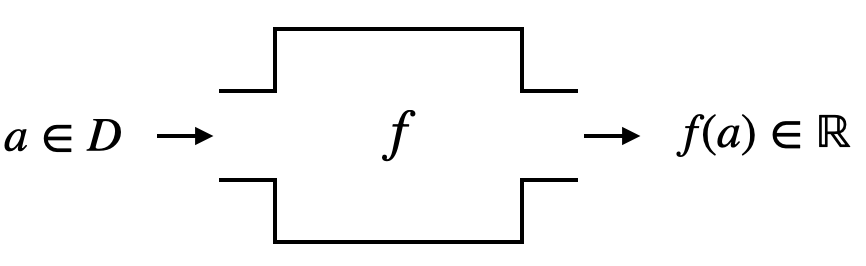
\includegraphics[width=60mm]{function.png}
 \end{center}
\end{figure}

\vspace{-2mm}

\end{frame}



%%%%%%%%%%%%%%%%%%%%%%%%%%%%%%%%%%%%%%%%%%%%%%%%%%%%%%%%%%%%%%%%%%%%%%%%%%%%%%%%%%%%%%%
%%%%%%%%%%%%%%%%%%%%%%%%%%%%%%%%%%%%%%%%%%%%%%%%%%%%%%%%%%%%%%%%%%%%%%%%%%%%%%%%%%%%%%%

\section{関数}

\begin{frame}
\frametitle{関数}   



例えば, 関数
$$
f: \R \longrightarrow \R, \ x \mapsto (1+x)^2
$$
はしばしば単に$f(x)=(1+x)^2$と書かれる. \\
\ \\

これは$a \in D=\R$に対して$(1+a)^2 \in \R$を返す「対応」だと考えられる. 
つまり
$$
f(-1)=0, \ \ \ f(0)=1, \ \ \ f(0.3)=1.69, \ \ \ f(10)=121
$$
といった具合である. \\
\ \\

$f$の像は$\R_{\ge 0}=\{x \in \R \ | \ x \ge 0\}$である. 

\end{frame}



%%%%%%%%%%%%%%%%%%%%%%%%%%%%%%%%%%%%%%%%%%%%%%%%%%%%%%%%%%%%%%%%%%%%%%%%%%%%%%%%%%%%%%%
%%%%%%%%%%%%%%%%%%%%%%%%%%%%%%%%%%%%%%%%%%%%%%%%%%%%%%%%%%%%%%%%%%%%%%%%%%%%%%%%%%%%%%%


\begin{frame}
\frametitle{関数のグラフ}   

$xy$-平面$\R^2$上の点$(x,f(x))$を考えることで, 関数$f$を可視化できる. 
集合
$$
\{(x,f(x)) \ | \ x \in D\} \subset \R^2
$$
を関数$f$の\underline{グラフ}という. 

\begin{figure}[htbp]
 \begin{center} 
  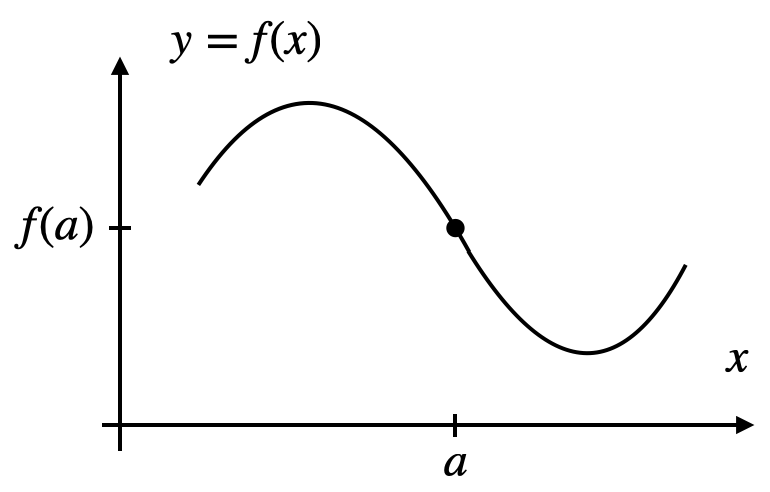
\includegraphics[width=60mm]{graph.png}
 \end{center}
\end{figure}


\end{frame}

%%%%%%%%%%%%%%%%%%%%%%%%%%%%%%%%%%%%%%%%%%%%%%%%%%%%%%%%%%%%%%%%%%%%%%%%%%%%%%%%%%%%%%%
%%%%%%%%%%%%%%%%%%%%%%%%%%%%%%%%%%%%%%%%%%%%%%%%%%%%%%%%%%%%%%%%%%%%%%%%%%%%%%%%%%%%%%%


\begin{frame}
\frametitle{関数のグラフ}   


\begin{figure}[htbp]
 \begin{center} 
  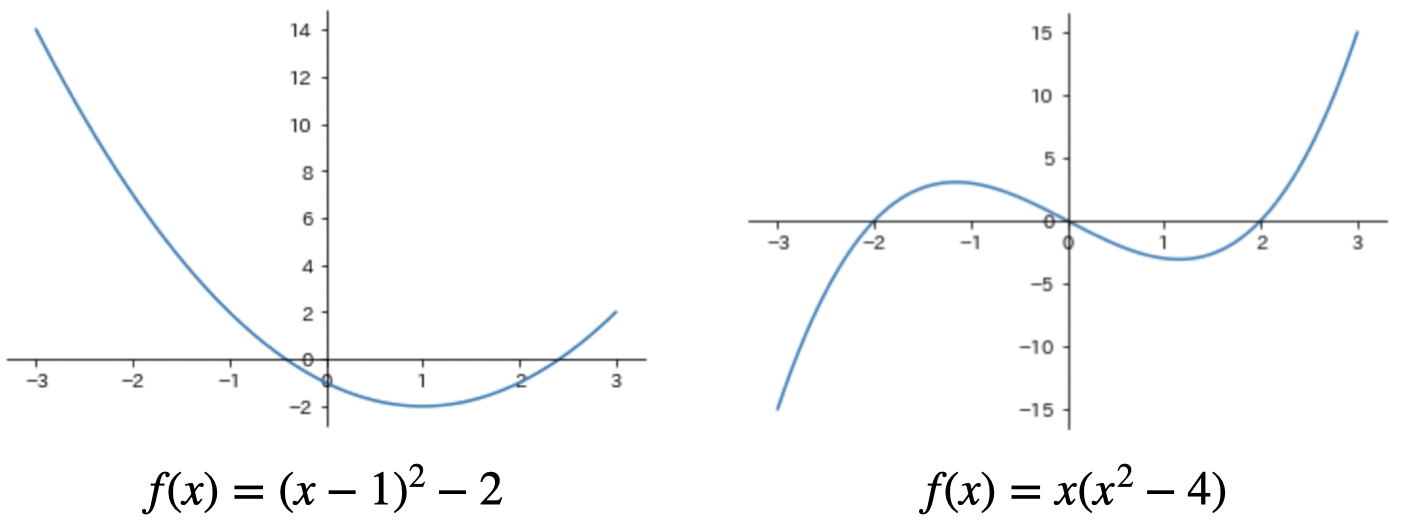
\includegraphics[width=100mm]{graph2.png}
 \end{center}
\end{figure}


\end{frame}


%%%%%%%%%%%%%%%%%%%%%%%%%%%%%%%%%%%%%%%%%%%%%%%%%%%%%%%%%%%%%%%%%%%%%%%%%%%%%%%%%%%%%%%
%%%%%%%%%%%%%%%%%%%%%%%%%%%%%%%%%%%%%%%%%%%%%%%%%%%%%%%%%%%%%%%%%%%%%%%%%%%%%%%%%%%%%%%


\begin{frame}
\frametitle{関数のグラフ}   


\begin{Prob}
次の関数のグラフを描け. 
\begin{enumerate}
\item $f(x)=2x-5$
\item $g(x)=x^2-2x-3$
\item $h(x)=|x^2-4x-12|$
\end{enumerate}
\end{Prob}


\end{frame}





%%%%%%%%%%%%%%%%%%%%%%%%%%%%%%%%%%%%%%%%%%%%%%%%%%%%%%%%%%%%%%%%%%%%%%%%%%%%%%%%%%%%%%%
%%%%%%%%%%%%%%%%%%%%%%%%%%%%%%%%%%%%%%%%%%%%%%%%%%%%%%%%%%%%%%%%%%%%%%%%%%%%%%%%%%%%%%%


\begin{frame}
\frametitle{関数の定義域}

次の2つの関数
\begin{align*}
f_1: \{ x \in \R \ | \ x \neq 0\} \longrightarrow \R, \ x \mapsto \frac{1}{x}\\
f_2: \{ x \in \R \ | \ x > 0\} \longrightarrow \R, \ x \mapsto \frac{1}{x}
\end{align*}
は定義域が異なるので, 厳密には異なる関数である. \\
\ \\

しかしながら, 特に言及がなければ$1/x$と書かれた関数は前者を指す. 
このように, 特に定義域を指定せずに式だけで与えられた関数は, その式に代入可能な実数全体を定義域とする関数と考える.


\end{frame}


%%%%%%%%%%%%%%%%%%%%%%%%%%%%%%%%%%%%%%%%%%%%%%%%%%%%%%%%%%%%%%%%%%%%%%%%%%%%%%%%%%%%%%%
%%%%%%%%%%%%%%%%%%%%%%%%%%%%%%%%%%%%%%%%%%%%%%%%%%%%%%%%%%%%%%%%%%%%%%%%%%%%%%%%%%%%%%%


\begin{frame}
\frametitle{関数の定義域}

\begin{itemize}
\item $x^2 + 3x$は$\R$上で定義された関数. 
\item $\frac{3x+1}{x^2-5}$は分母が$0$にならない範囲, つまり$x\neq \pm \sqrt{5}$で定義された関数. 
\item $\sqrt{x-3}$は平方根の中身が非負である範囲, つまり$x\ge 3$で定義された関数. 
\end{itemize}
%定義域が$\R$である関数を\underline{全実数}という. 

\end{frame}


%%%%%%%%%%%%%%%%%%%%%%%%%%%%%%%%%%%%%%%%%%%%%%%%%%%%%%%%%%%%%%%%%%%%%%%%%%%%%%%%%%%%%%%
%%%%%%%%%%%%%%%%%%%%%%%%%%%%%%%%%%%%%%%%%%%%%%%%%%%%%%%%%%%%%%%%%%%%%%%%%%%%%%%%%%%%%%%

\section{多項式関数}


\begin{frame}
\frametitle{多項式関数}

\begin{itemize}
\item 
$a_0,a_1,\dots,a_n \in \R$に対して, 
$$
f(x)=a_nx^n+a_{n-1}x^{n-1}+\dots+a_1x+a_0
$$
の形の関数を\underline{多項式関数}という. 
\item 例
$$
-2x+3, \ \ \ x^3-x^2+7x+10, \ \ \ x^{100} 
$$
\item $a_i$は$x^i$の\underline{係数}, $a_0$は\underline{定数項}と呼ばれる. 
\item $a_n \neq 0$であるとき, $n$を$f(x)$の\underline{次数}, $f(x)$を$n$次多項式関数という. 
\item 多項式関数の定義域は$\R$. 
\end{itemize}

\end{frame}



%%%%%%%%%%%%%%%%%%%%%%%%%%%%%%%%%%%%%%%%%%%%%%%%%%%%%%%%%%%%%%%%%%%%%%%%%%%%%%%%%%%%%%%
%%%%%%%%%%%%%%%%%%%%%%%%%%%%%%%%%%%%%%%%%%%%%%%%%%%%%%%%%%%%%%%%%%%%%%%%%%%%%%%%%%%%%%%


\section{有理関数}

\begin{frame}
\frametitle{有理関数}

\begin{itemize}
\item 
多項式関数$f(x),g(x)$の有理式, つまり
$$
h(x)=\frac{f(x)}{g(x)}
$$
の形で書かれる関数を\underline{有理関数}という. 
\item 例
$$
\frac{1}{x+1}, \ \ \ \frac{1}{x}+\frac{1}{x+1}, \ \ \ \frac{(x-1)(x+5)}{(x-3)(x+1)(x-7)}
$$
\item 多項式関数は有理関数の特別な場合($g(x)=1$の場合). 
\item 有理関数の定義域は$D=\{ x \in \R \ | g(x) \neq 0\}$.
\end{itemize}
%(共通因子に関しては, 後で詳しく議論する.)

\end{frame}


%%%%%%%%%%%%%%%%%%%%%%%%%%%%%%%%%%%%%%%%%%%%%%%%%%%%%%%%%%%%%%%%%%%%%%%%%%%%%%%%%%%%%%%
%%%%%%%%%%%%%%%%%%%%%%%%%%%%%%%%%%%%%%%%%%%%%%%%%%%%%%%%%%%%%%%%%%%%%%%%%%%%%%%%%%%%%%%


\section{無理関数}

\begin{frame}
\frametitle{無理関数}

\begin{itemize}
\item 
多項式と根号の有理式で表され, 変数が根号に含まれる関数を\underline{無理関数}という. 
\item 例
$$
\sqrt{x^2-1}+x^3+\frac{5}{2}, \ \ \ \frac{\sqrt{x}}{x-1}+2, \ \ \ \sqrt[3]{\frac{x^2+x+1}{5x^2-7}}+100x
$$
\item 無理関数の定義域は一般に複雑である. 例えば, 上の関数の定義域はそれぞれ
$$
\{x \in \R \ | \ x^2 \ge 1\}, \ \ \ \{x \in \R \ | \ x \ge 0, x \neq 1\}, \ \ \ \{x \in \R \ | \ x \neq \pm \sqrt{7/5}\}
$$
\end{itemize}

\end{frame}


%%%%%%%%%%%%%%%%%%%%%%%%%%%%%%%%%%%%%%%%%%%%%%%%%%%%%%%%%%%%%%%%%%%%%%%%%%%%%%%%%%%%%%%
%%%%%%%%%%%%%%%%%%%%%%%%%%%%%%%%%%%%%%%%%%%%%%%%%%%%%%%%%%%%%%%%%%%%%%%%%%%%%%%%%%%%%%%

\section{三角関数}


\begin{frame}
\frametitle{三角関数}

\begin{itemize}
\item 
\underline{三角関数}: 平面三角法の角度と線分長の関係を記述する関数の族, 及びそれらを拡張して得られる関数の総称. 
\item 正弦関数$\sin \theta$, 余弦関数$\cos \theta$, 正接関数$\tan \theta= \sin \theta / \cos \theta$が代表的. 
\item 大学では, 変数$\theta$の単位として, 度数法(度)ではなく弧度法(radian)を考えることが多い. 
$1$ radian: ``半径=弧長"なる角度. 
\item $2\pi$ rad = $360^\circ$, つまり$1$ rad =  $360^\circ/2 \pi \approx 57.3 ^\circ$. 
\end{itemize}

\vspace{-2mm}

\begin{figure}[htbp]
 \begin{center} 
  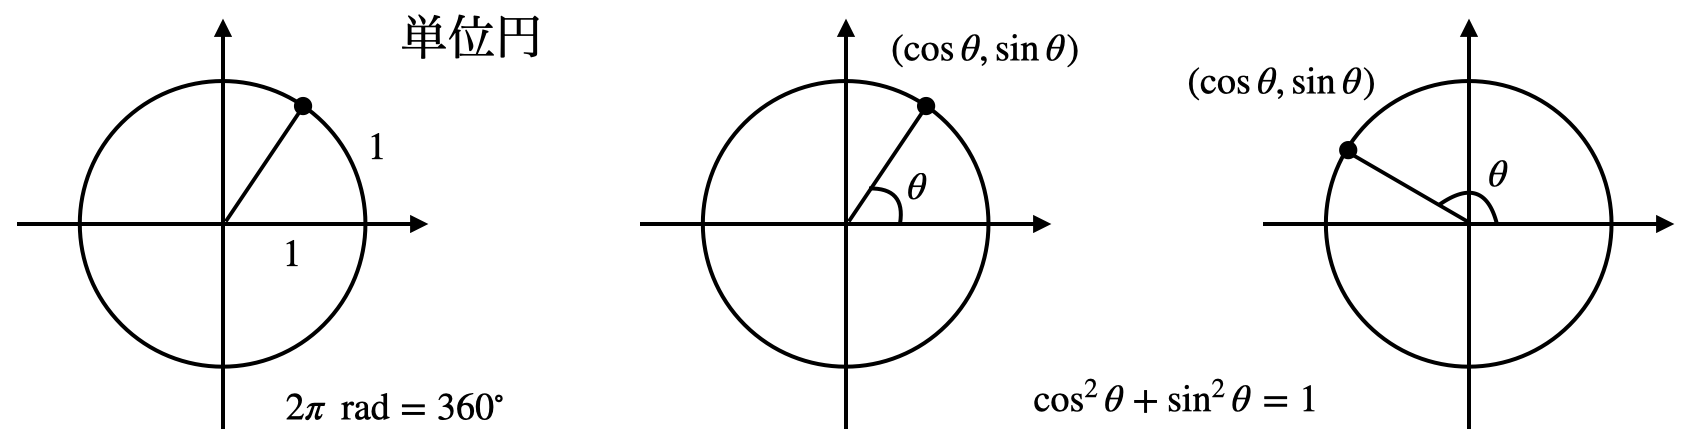
\includegraphics[width=115mm]{radian.png}
 \end{center}
\end{figure}
\vspace{-2mm}

\end{frame}




%%%%%%%%%%%%%%%%%%%%%%%%%%%%%%%%%%%%%%%%%%%%%%%%%%%%%%%%%%%%%%%%%%%%%%%%%%%%%%%%%%%%%%%
%%%%%%%%%%%%%%%%%%%%%%%%%%%%%%%%%%%%%%%%%%%%%%%%%%%%%%%%%%%%%%%%%%%%%%%%%%%%%%%%%%%%%%%




\begin{frame}
\frametitle{三角関数}

$0 <\theta <\pi/2$であるとき

%\vspace{-2mm}
\begin{figure}[htbp]
 \begin{center} 
  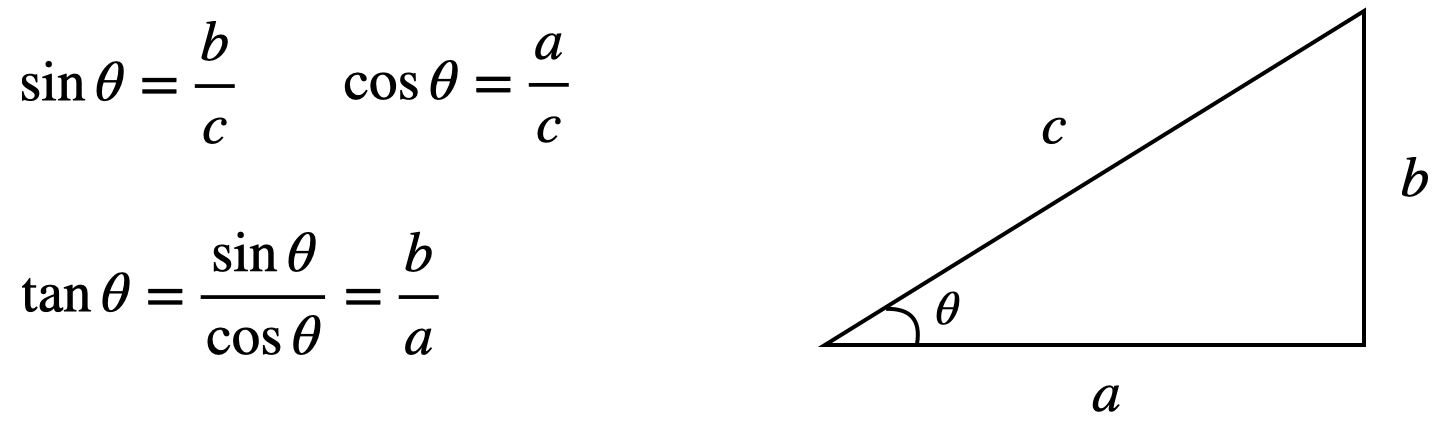
\includegraphics[width=90mm]{sin_cos_tan.png}
 \end{center}
\end{figure}
%\vspace{-4mm}

具体的には
\begin{itemize}
\item $\sin(\pi/6)=1/2$, $\sin(\pi/4)=1/\sqrt{2}$, $\sin(\pi/3) =\sqrt{3}/2$, 
\item $\cos(\pi/6)=\sqrt{3}/2$, $\cos(\pi/4)=1/\sqrt{2}$, $\cos(\pi/3)=1/2$
\item  $\tan(pi/6)=1/\sqrt{3}$, $\tan(\pi/4)=1$, $\tan(\pi/3)=\sqrt{3}$
\end{itemize}


\end{frame}



%%%%%%%%%%%%%%%%%%%%%%%%%%%%%%%%%%%%%%%%%%%%%%%%%%%%%%%%%%%%%%%%%%%%%%%%%%%%%%%%%%%%%%%
%%%%%%%%%%%%%%%%%%%%%%%%%%%%%%%%%%%%%%%%%%%%%%%%%%%%%%%%%%%%%%%%%%%%%%%%%%%%%%%%%%%%%%%




\begin{frame}
\frametitle{三角関数の性質}

\begin{itemize}
\item 周期: $\sin (x + 2\pi) = \sin x$, $\cos (x + 2\pi) = \cos x$, $\tan (x +\pi) = \tan x$
\item $\sin(\alpha+\beta)=\sin \alpha \cos \beta + \cos \alpha \sin \beta$
\item $\cos(\alpha+\beta)=\cos \alpha \cos \beta - \sin \alpha \sin \beta$
\end{itemize}

\vspace{-2mm}

\begin{figure}[htbp]
 \begin{center} 
  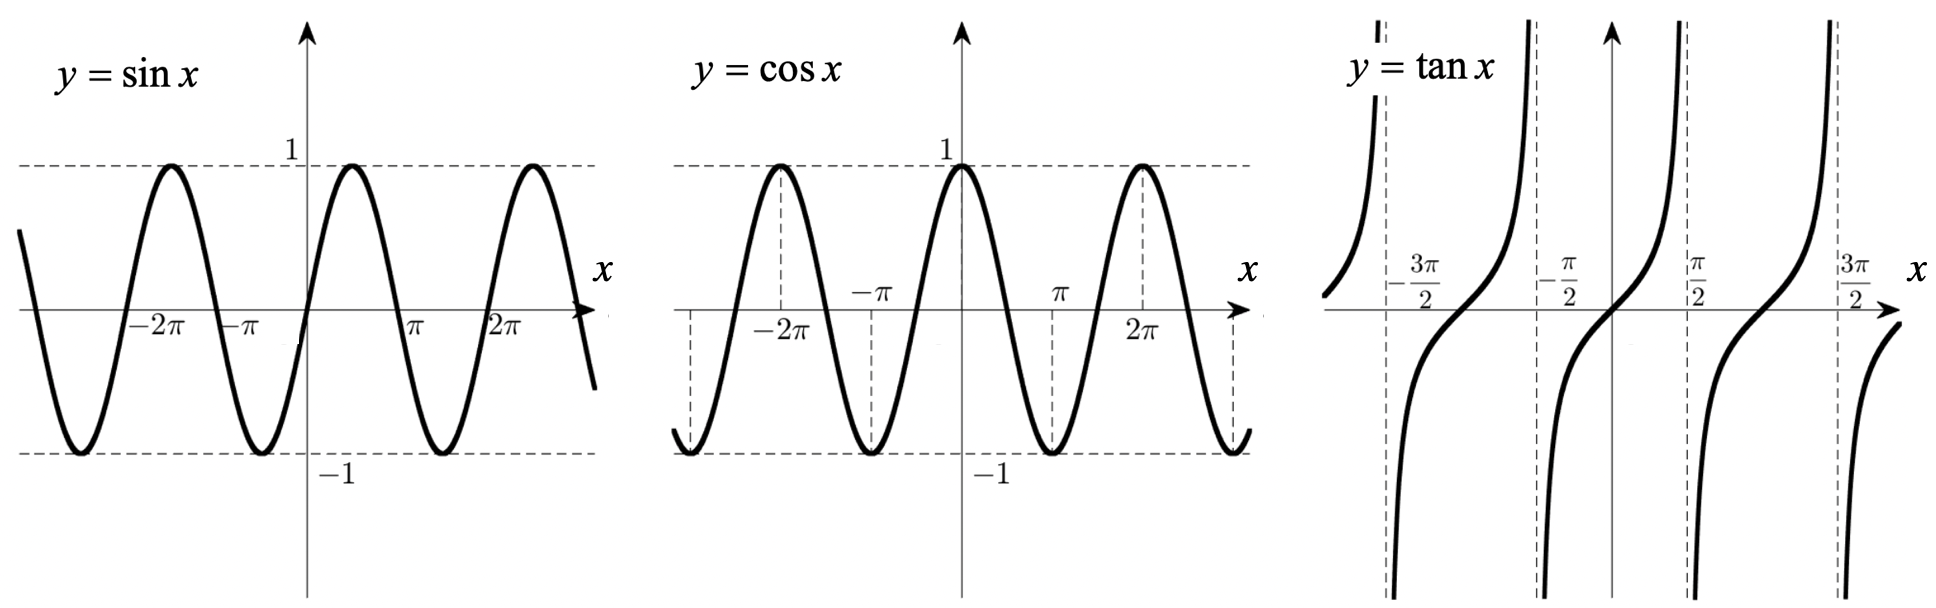
\includegraphics[width=122mm]{trig.png}
 \end{center}
\end{figure}
\vspace{-4mm}

\end{frame}



%%%%%%%%%%%%%%%%%%%%%%%%%%%%%%%%%%%%%%%%%%%%%%%%%%%%%%%%%%%%%%%%%%%%%%%%%%%%%%%%%%%%%%%
%%%%%%%%%%%%%%%%%%%%%%%%%%%%%%%%%%%%%%%%%%%%%%%%%%%%%%%%%%%%%%%%%%%%%%%%%%%%%%%%%%%%%%%




\begin{frame}
\frametitle{三角関数の性質}

\begin{Prob}
三角関数$\sin x$, $\cos x$, $\tan x$の定義域と像を求めよ.  
\end{Prob}

\begin{Prob}
次の関数のグラフを描け. 
\begin{enumerate}
\item $3\sin(2x)$
\item $\cos(x+\frac{\pi}{3})$ + 1
\end{enumerate}
\end{Prob}

一般に, $a,b,c,d \in \R$に対して, $af(bx+c)+d$のグラフは$f(x)$のグラフを$x$軸方向に$1/b$倍し, $c$だけ左にずらし, $y$軸方向に$a$倍し, $d$だけ上にずらしたもの. 
\end{frame}


%%%%%%%%%%%%%%%%%%%%%%%%%%%%%%%%%%%%%%%%%%%%%%%%%%%%%%%%%%%%%%%%%%%%%%%%%%%%%%%%%%%%%%%
%%%%%%%%%%%%%%%%%%%%%%%%%%%%%%%%%%%%%%%%%%%%%%%%%%%%%%%%%%%%%%%%%%%%%%%%%%%%%%%%%%%%%%%

\section{指数関数}


\begin{frame}
\frametitle{指数関数}

\begin{itemize}
\item  $n\in \N$, $a >0$に対して, 冪乗$a^n =\overbrace{ a \times a \times \dots \times a}^\text{$n$個}$であった. 
$a$は\underline{底}, $n$は\underline{指数}と呼ばれる. 
さらに$a^{-n}=1/a^n$, $a^0=1$と定めることで, 指数が整数の場合にも冪乗が定義される. 
\item 例
$$
2^5=32, \ \ \ 2^{-4}=\frac{1}{16}, \ \ 2^0=1. 
$$
\item 有理数$x \in \Q$に対して, $a$の冪乗$a^x$を次のように定義する. 
$m \in \N$, $n\in \Z$, $a>0$に対して, 
$$
a^{\frac{n}{m}}=\sqrt[m]{a^n} \ (=(\sqrt[m]{a})^n). 
$$
\item 例
$$
5^{\frac{2}{3}}=\sqrt[3]{5^2} \approx 2.924,  \ \ \ 2^{-\frac{3}{4}}=2^{\frac{-3}{4}}=\sqrt[4]{1/2^3} \approx 0.5946.  
$$
\end{itemize}



\end{frame}


%%%%%%%%%%%%%%%%%%%%%%%%%%%%%%%%%%%%%%%%%%%%%%%%%%%%%%%%%%%%%%%%%%%%%%%%%%%%%%%%%%%%%%%
%%%%%%%%%%%%%%%%%%%%%%%%%%%%%%%%%%%%%%%%%%%%%%%%%%%%%%%%%%%%%%%%%%%%%%%%%%%%%%%%%%%%%%%




\begin{frame}
\frametitle{指数関数}

\begin{itemize}
\item 上の考察を元にして$x \in \R$に対して$a^x \in \R$が定義される. (厳密には有理数の稠密性を議論する必要があるが省略)
\item 関数$f(x)=a^x$を$a$を底とする\underline{指数関数}という, 
\item ネイピア数$e=2.7182\dots$を底とする場合が多い. 
\end{itemize}


\vspace{-1mm}

\begin{figure}[htbp]
 \begin{center} 
  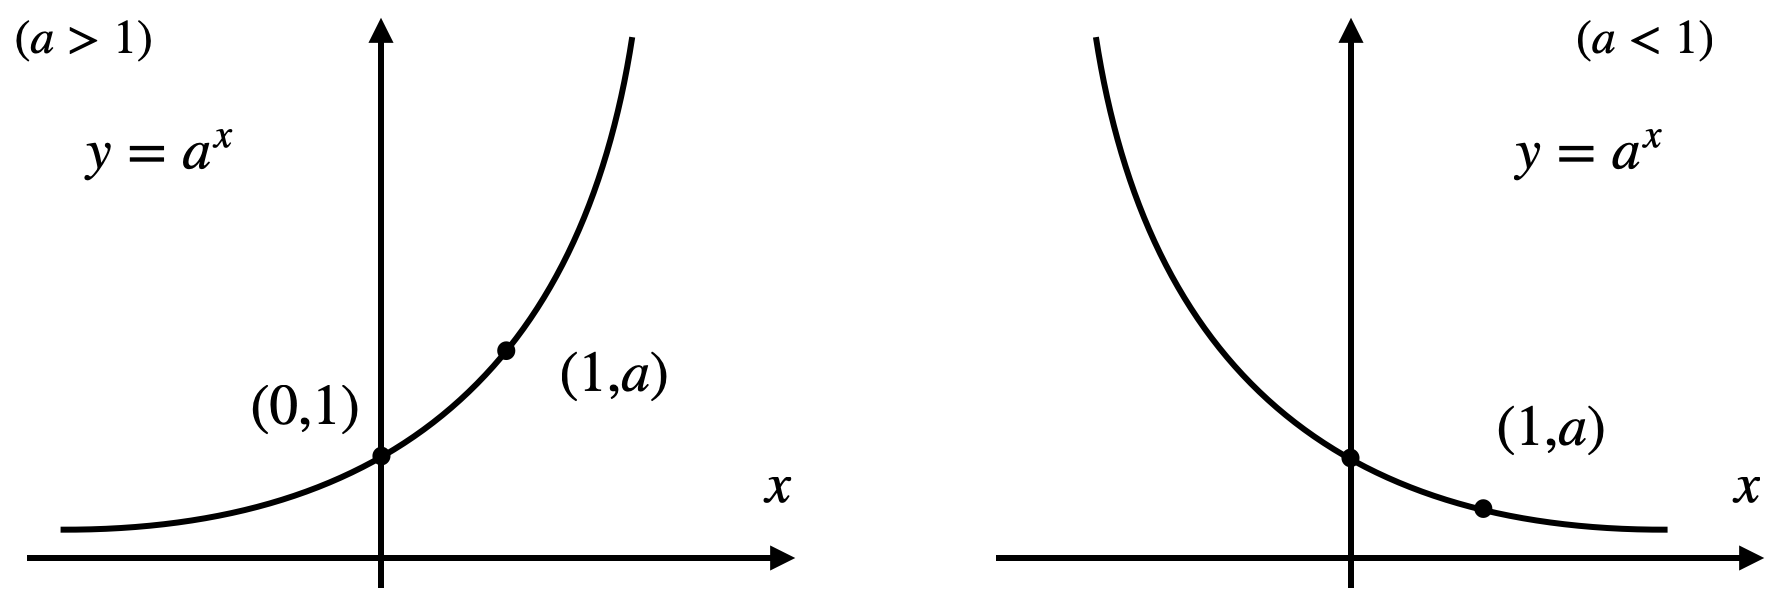
\includegraphics[width=100mm]{exp.png}
 \end{center}
\end{figure}
\vspace{-4mm}


\end{frame}




%%%%%%%%%%%%%%%%%%%%%%%%%%%%%%%%%%%%%%%%%%%%%%%%%%%%%%%%%%%%%%%%%%%%%%%%%%%%%%%%%%%%%%%
%%%%%%%%%%%%%%%%%%%%%%%%%%%%%%%%%%%%%%%%%%%%%%%%%%%%%%%%%%%%%%%%%%%%%%%%%%%%%%%%%%%%%%%

\section{対数関数}

\begin{frame}
\frametitle{対数関数}   

\begin{itemize}
\item 
$a \ne 1$を正の実数とすると, 任意の$x \in \R_+$に対して
$$
x=a^y
$$
を満たす$y \in \R$が唯一つ存在する. これを$y=\log_a x$と書き, $a$を底とする$x$の\underline{対数}という. 
\item $f(x)=\log_a x$を$a$を底とする\underline{対数関数}という. 
定義域が$\R_+$であることに注意($f: \R_{+} \rightarrow \R, x \mapsto \log_a x$).   
\end{itemize}

例
$$
 \log_2 \frac{1}{2}=-1, \  \log_2 1=0, \ \log_2 2=1, \  \log_2 4=2, \  \log_2 8=3, \  \log_2 16=4
$$
($2^{-1}=1/2$, $2^{0}=1$, $2^{1}=2$, $2^{2}=4$, $2^{3}=8$, $2^{4}=16$)


\end{frame}



%%%%%%%%%%%%%%%%%%%%%%%%%%%%%%%%%%%%%%%%%%%%%%%%%%%%%%%%%%%%%%%%%%%%%%%%%%%%%%%%%%%%%%%
%%%%%%%%%%%%%%%%%%%%%%%%%%%%%%%%%%%%%%%%%%%%%%%%%%%%%%%%%%%%%%%%%%%%%%%%%%%%%%%%%%%%%%%


\begin{frame}
\frametitle{対数関数}   

\begin{itemize}
\item 定義より, $a^{\log_a x}=x$, $\log_a a=1$, $\log_a 1=0$. 
\item 特別な底に関して, 対数は特別な名前を持つ: 
\begin{enumerate}
\item 常用対数: $\log_{10} x=\mathrm{Log} x$, 
\item 自然対数: $\log_e x=\log x, \ln x$, 
\item 二進対数: $\log_2 x$.  
\end{enumerate}
\end{itemize}

\vspace{-1mm}

\begin{figure}[htbp]
 \begin{center} 
  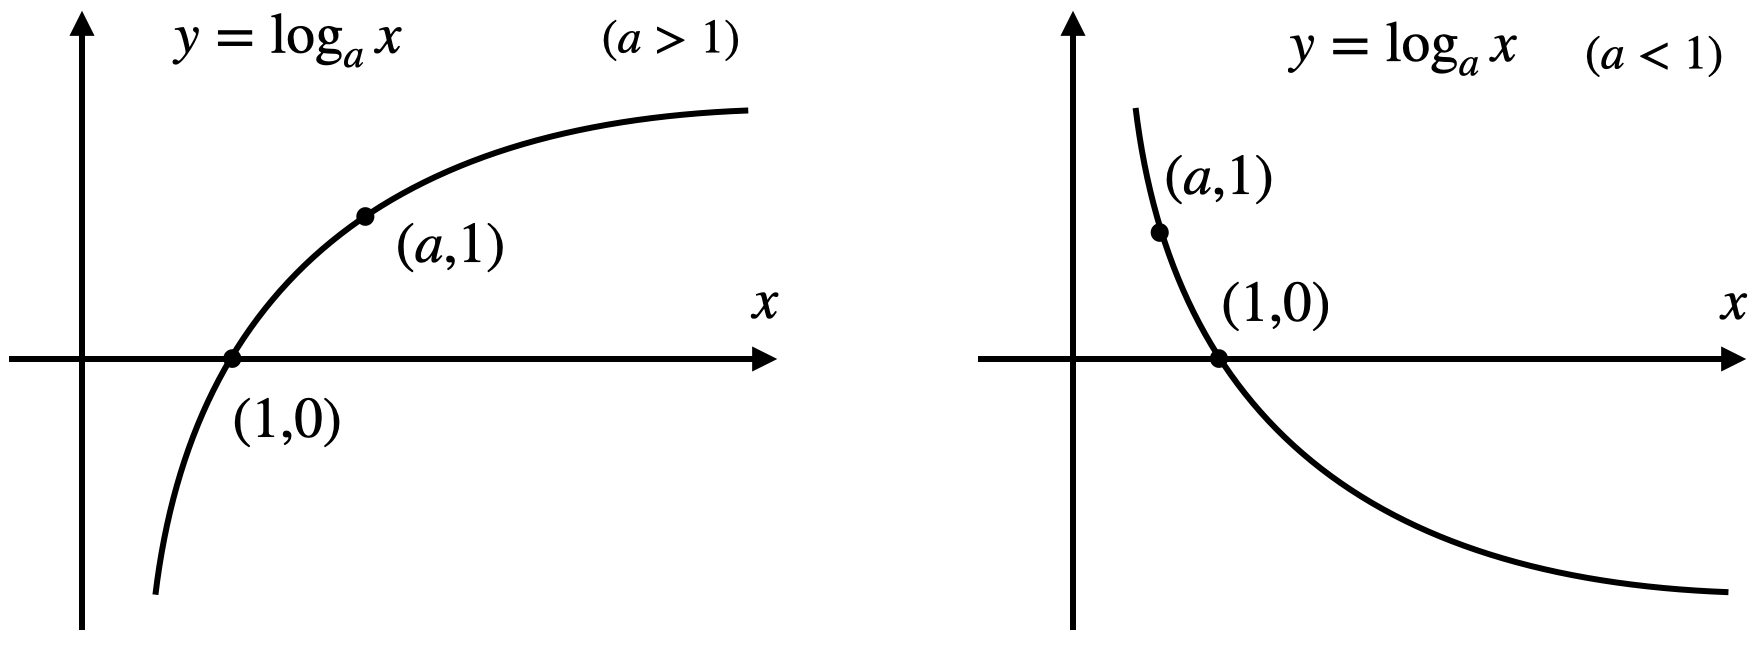
\includegraphics[width=100mm]{log.png}
 \end{center}
\end{figure}
\vspace{-4mm}

\end{frame}



%%%%%%%%%%%%%%%%%%%%%%%%%%%%%%%%%%%%%%%%%%%%%%%%%%%%%%%%%%%%%%%%%%%%%%%%%%%%%%%%%%%%%%%
%%%%%%%%%%%%%%%%%%%%%%%%%%%%%%%%%%%%%%%%%%%%%%%%%%%%%%%%%%%%%%%%%%%%%%%%%%%%%%%%%%%%%%%


\begin{frame}
\frametitle{対数関数}   


\begin{Thm}
\begin{itemize}
\item $\log_a xy= \log_a x + \log_a y$
\item $\log_a x^b = b \log_a x$
\item (底の変換公式) 正の実数$a,b(\ne1)$と$x$に対して
$$
\log_a x = \frac{\log_b x}{\log_b a}. 
$$
\end{itemize}
\end{Thm}

例
\begin{itemize}
\item $\log_2 10 = \log_2 2+\log_2 5 =1+ \log_2 5$, 
\item $\log_3 12= \log_3 3 + \log_3 2^2=1+2 \log_3 2$, 
\item $\log_5 \frac{15}{4} = \log_5 15 +\log_5 \frac{1}{2^2} = 1+ \log_5 3 - 2\log_5 2$, 
\item $\log_7 5= \log_2 5 / \log_2 7$. 
\end{itemize}


\end{frame}



%%%%%%%%%%%%%%%%%%%%%%%%%%%%%%%%%%%%%%%%%%%%%%%%%%%%%%%%%%%%%%%%%%%%%%%%%%%%%%%%%%%%%%%
%%%%%%%%%%%%%%%%%%%%%%%%%%%%%%%%%%%%%%%%%%%%%%%%%%%%%%%%%%%%%%%%%%%%%%%%%%%%%%%%%%%%%%%

\section{指数関数と対数関数}

\begin{frame}
\frametitle{指数関数と対数関数}   

\begin{itemize}
\item $a \ne 1$に関して, 指数関数$f(x)=a^x$の像は$\R_+$, 対数関数$g(x)=\log_ax$の定義域は$\R_+$. 
\item $f(x)$と$g(x)$は互いに\underline{逆関数}(逆写像);  
$$
g(f(x))=\log_a(a^x)=x, \ \ \ f(g(x))=a^{\log_ax}=x. 
$$
\end{itemize}

\vspace{-1mm}

\begin{figure}[htbp]
 \begin{center} 
  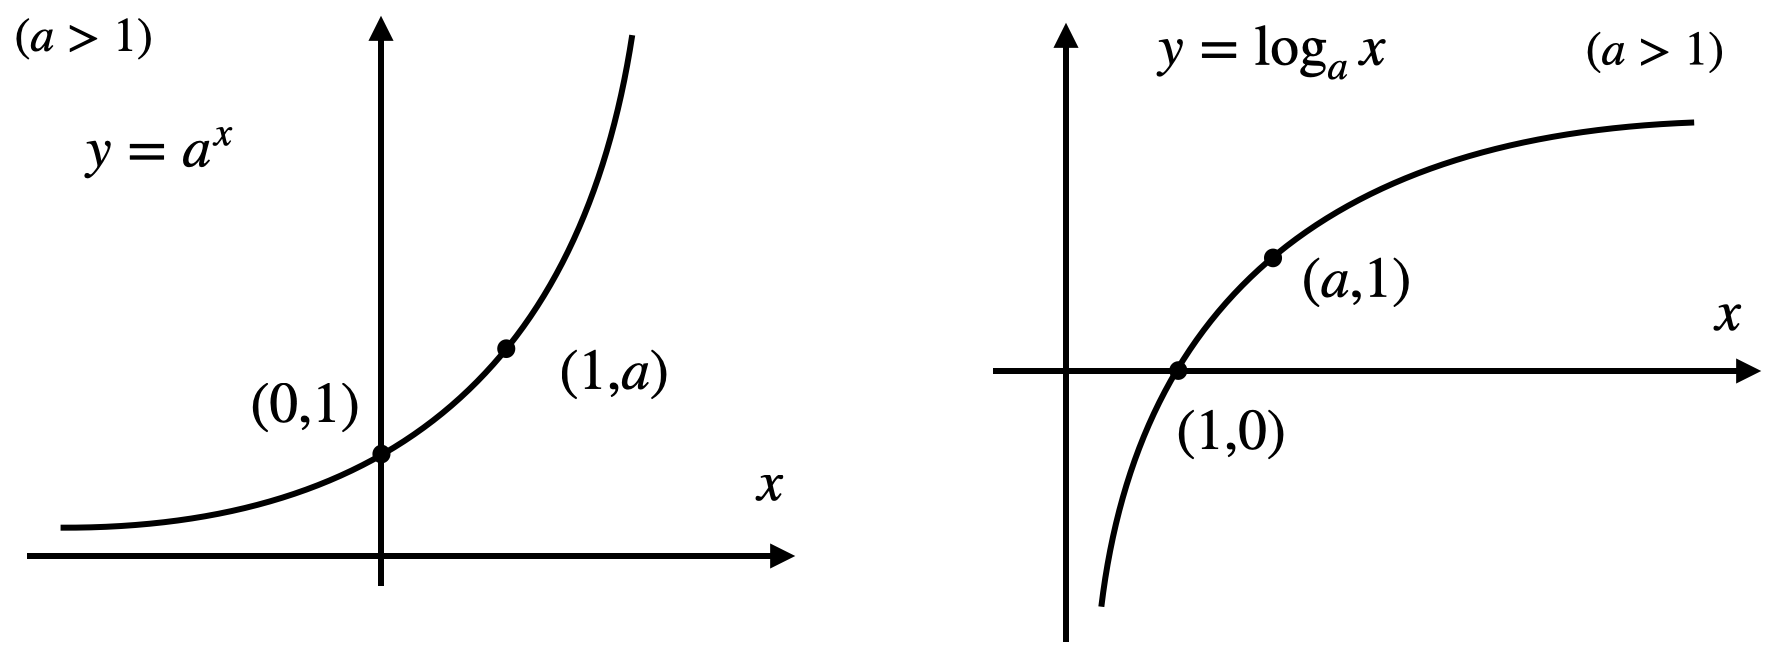
\includegraphics[width=100mm]{exp_log.png}
 \end{center}
\end{figure}
\vspace{-4mm}

(一般に, 逆写像のグラフは$x=y$に関して鏡映対称)

\end{frame}

%%%%%%%%%%%%%%%%%%%%%%%%%%%%%%%%%%%%%%%%%%%%%%%%%%%%%%%%%%%%%%%%%%%%%%%%%%%%%%%%%%%%%%%
%%%%%%%%%%%%%%%%%%%%%%%%%%%%%%%%%%%%%%%%%%%%%%%%%%%%%%%%%%%%%%%%%%%%%%%%%%%%%%%%%%%%%%%


\section{符号関数}

\begin{frame}
\frametitle{符号関数}   

符号関数
$$
\mathrm{sgn}(x) = 
\begin{cases}
\frac{|x|}{x} & (x \ne 0) \\
0 & (x =0)
 \end{cases} \ \ 
 =
\begin{cases}
1 & (x > 0) \\
0 & (x =0) \\
-1 & (x<0)
 \end{cases}
$$

\vspace{-1mm}

\begin{figure}[htbp]
 \begin{center} 
  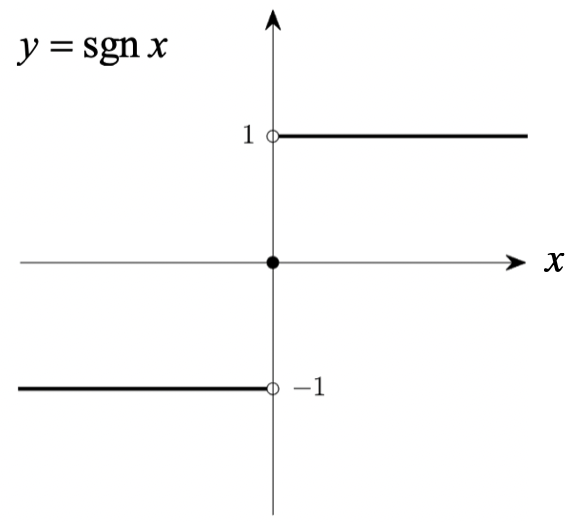
\includegraphics[width=45mm]{sgn.png}
 \end{center}
\end{figure}
\vspace{-4mm}

\end{frame}



%%%%%%%%%%%%%%%%%%%%%%%%%%%%%%%%%%%%%%%%%%%%%%%%%%%%%%%%%%%%%%%%%%%%%%%%%%%%%%%%%%%%%%%
%%%%%%%%%%%%%%%%%%%%%%%%%%%%%%%%%%%%%%%%%%%%%%%%%%%%%%%%%%%%%%%%%%%%%%%%%%%%%%%%%%%%%%%




\begin{frame}
\frametitle{符号関数}   

\begin{Prob}
次の関数のグラフを描け. 
\begin{enumerate}
\item $\mathrm{sgn}(x^2)$, $\mathrm{sgn}(x^3)$
\item $\frac{x+|x|}{2x} \ \ \ (x \neq 0)$. 
\end{enumerate}
\end{Prob}
最後の関数はヘヴィサイドの階段関数と呼ばれる. 


\end{frame}




%%%%%%%%%%%%%%%%%%%%%%%%%%%%%%%%%%%%%%%%%%%%%%%%%%%%%%%%%%%%%%%%%%%%%%%%%%%%%%%%%%%%%%%
%%%%%%%%%%%%%%%%%%%%%%%%%%%%%%%%%%%%%%%%%%%%%%%%%%%%%%%%%%%%%%%%%%%%%%%%%%%%%%%%%%%%%%%

\section{床関数と天井関数}


\begin{frame}
\frametitle{床関数}   


床関数$\left \lfloor{x}\right \rfloor $
$$
\left \lfloor{x}\right \rfloor = \max\{ n \in \Z \ | \ x \ge n\}
$$
例
$$
\left \lfloor{1/2}\right \rfloor=0, \ \ \  \left \lfloor{-\pi}\right \rfloor=-4, \ \ \ \left \lfloor{5}\right \rfloor=5,  \ \ \ \left \lfloor{5.1}\right \rfloor=5
$$

\vspace{-1mm}

\begin{figure}[htbp]
 \begin{center} 
  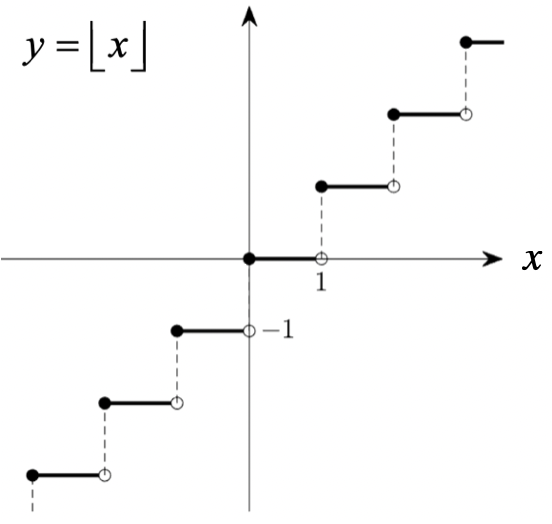
\includegraphics[width=45mm]{floor.png}
 \end{center}
\end{figure}
\vspace{-4mm}

\end{frame}



%%%%%%%%%%%%%%%%%%%%%%%%%%%%%%%%%%%%%%%%%%%%%%%%%%%%%%%%%%%%%%%%%%%%%%%%%%%%%%%%%%%%%%%
%%%%%%%%%%%%%%%%%%%%%%%%%%%%%%%%%%%%%%%%%%%%%%%%%%%%%%%%%%%%%%%%%%%%%%%%%%%%%%%%%%%%%%%




\begin{frame}
\frametitle{天井関数}   


天井関数$\left \lceil{x}\right \rceil$
$$
\left \lceil{x}\right \rceil = \min\{ n \in \Z \ | \ x \le n\}
$$
例
$$
\left \lceil{1/2}\right \rceil =1, \ \ \  \left \lceil{-\pi}\right \rceil =-3, \ \ \ \left \lceil{5}\right \rceil =5,  \ \ \ \left \lceil{5.1}\right \rceil =6
$$

\vspace{-1mm}

\begin{figure}[htbp]
 \begin{center} 
  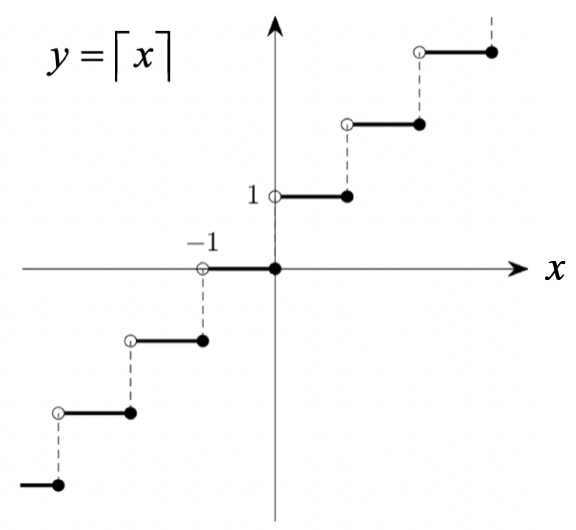
\includegraphics[width=45mm]{ceiling.png}
 \end{center}
\end{figure}
\vspace{-4mm}

\end{frame}


%%%%%%%%%%%%%%%%%%%%%%%%%%%%%%%%%%%%%%%%%%%%%%%%%%%%%%%%%%%%%%%%%%%%%%%%%%%%%%%%%%%%%%%
%%%%%%%%%%%%%%%%%%%%%%%%%%%%%%%%%%%%%%%%%%%%%%%%%%%%%%%%%%%%%%%%%%%%%%%%%%%%%%%%%%%%%%%




\begin{frame}
\frametitle{床関数と天井関数}   


床関数$\left \lfloor{x}\right \rfloor $, 天井関数$\left \lceil{x}\right \rceil$
$$
\left \lfloor{x}\right \rfloor = \max\{ n \in \Z \ | \ x \ge n\}, \ \ \ \left \lceil{x}\right \rceil = \min\{ n \in \Z \ | \ x \le n\}
$$

\vspace{-1mm}

\begin{figure}[htbp]
 \begin{center} 
  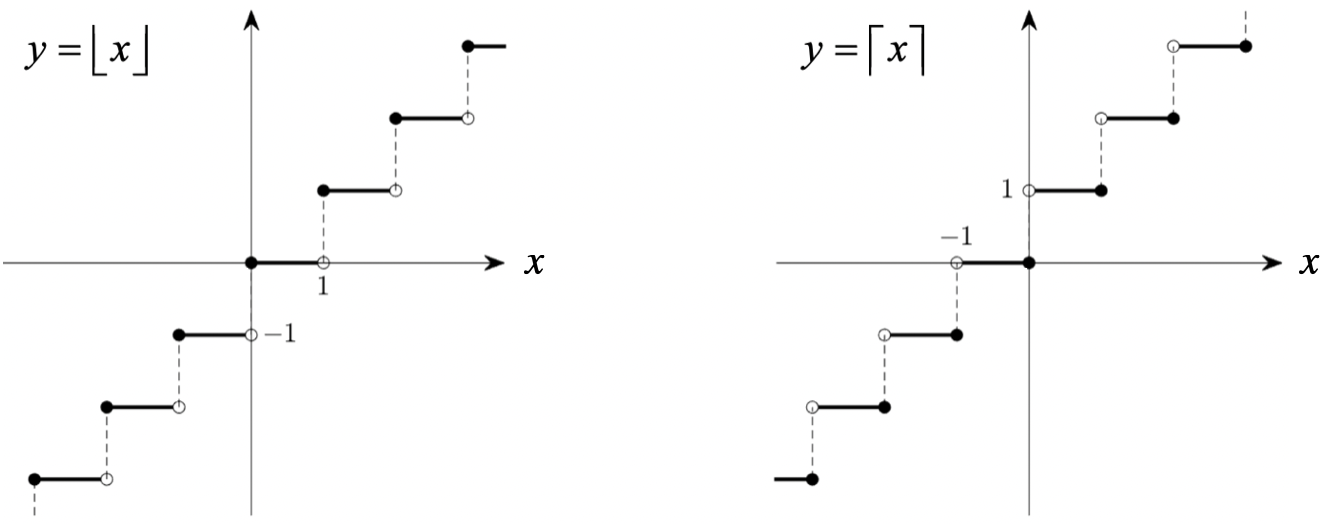
\includegraphics[width=100mm]{floor_ceiling.png}
 \end{center}
\end{figure}
\vspace{-4mm}

\end{frame}



%%%%%%%%%%%%%%%%%%%%%%%%%%%%%%%%%%%%%%%%%%%%%%%%%%%%%%%%%%%%%%%%%%%%%%%%%%%%%%%%%%%%%%%
%%%%%%%%%%%%%%%%%%%%%%%%%%%%%%%%%%%%%%%%%%%%%%%%%%%%%%%%%%%%%%%%%%%%%%%%%%%%%%%%%%%%%%%




\begin{frame}
\frametitle{様々な関数のグラフ}   

\begin{Prob}
次の関数のグラフを描け. 
\begin{enumerate}
\item $\mathrm{sgn}(\sin x)$
\item $\left \lfloor{\frac{1}{2}x+1}\right \rfloor $
\end{enumerate}
\end{Prob}

\end{frame}



%%%%%%%%%%%%%%%%%%%%%%%%%%%%%%%%%%%%%%%%%%%%%%%%%%%%%%%%%%%%%%%%%%%%%%%%%%%%%%%%%%%%%%%
%%%%%%%%%%%%%%%%%%%%%%%%%%%%%%%%%%%%%%%%%%%%%%%%%%%%%%%%%%%%%%%%%%%%%%%%%%%%%%%%%%%%%%%




\section{今日のまとめ}
\begin{frame}
\frametitle{まとめ}   


\begin{enumerate}
\item 関数 (写像との関係, グラフ, 定義域)
\item 多項式関数, 有理関数, 無理関数, 三角関数, 指数関数, 対数関数
\item 符号関数, 床関数, 天井関数
\end{enumerate} 


\end{frame}


\end{document}